\documentclass{article}
\usepackage[utf8]{inputenc}
\usepackage{geometry}
\usepackage[export]{adjustbox}
\geometry{top=2cm, bottom=2cm, left=1.5cm, right=1.5cm}
\usepackage{titlesec}
\usepackage{lipsum}
\usepackage{fancyhdr}
\usepackage{enumitem}
\usepackage{hyperref}
\hypersetup{colorlinks=true,  linkcolor=black, citecolor=black, urlcolor=blue}
\hypersetup{pdfborder=0 0 0}
\usepackage{graphicx}
\usepackage{caption}
\usepackage{subcaption}
\usepackage{dirtytalk}

\usepackage[ngerman]{babel}
\usepackage{pythonhighlight}


\title{\textbf {Inwieweit nimmt Elon Musk durch sein Verhalten auf der Social-Media-Plattform X (ehem. Twitter) Einfluss auf den Kursverlauf von Tesla und Dogecoin?}}

\author{Eine Analyse und Bewertung der Big Data Bandits \\ (Daniel Linck, Daniel Weißenberger, David Helwich, Jonas Sigmund)}
\date{\today}

\begin{document}


\maketitle

\tableofcontents
\newpage

\section{Einleitung} \label{Einleitung}
Da gerade das digitale Zeitalter geprägt von dem Einfluss großer Social-Media-Plattformen ist, haben die Big Data Bandits beschlossen, im Rahmen der Klausuraufgabe diese Extremen genauer zu betrachten.
Unter dem Aspekt, dass Elon Musk wohl zu den populärsten, einflussreichsten und dominantesten Personen des öffentlichen Lebens zählt, nominiert ihn insbesondere sein einzigartiges Korrespondenzverhalten gepaart mit seinen wirtschaftlichen Interessen für eine genauere Untersuchung.
Im folgenden Abstract findet eine Analyse und Beantwortung der Fragestellung im Rahmen der gestellten Klausuraufgabe statt.
Dafür analysieren wir die entsprechenden Datensätze mit einem für diese Aufgabe entwickelten Python Script.
Dieses kann, aufgrund seiner hohen Modularität, auch in der Zukunft zur Beantwortung ähnlicher Fragestellungen verwendet werden.
Weitere Details bezüglich des Codes können der \href{https://github.com/alphaname007/BigDataBandits/blob/19beac1a6b5469aed05b4a6c072883810df6aacd/code\_main.ipynb}{code\_main.ipynb} entnommen werden.
Wir empfehlen zumindest einen kurzen Überflug über diese Datei, um die Transparenz und Sorgfalt der Analyse selbst beurteilen zu können.


\section{Fragestellung} \label{Fragestellung}
Die Fragestellung: ``Inwieweit nimmt Elon Musk durch sein Verhalten auf der Social-Media-Plattform X (ehem. Twitter) Einfluss auf den Kursverlauf von Tesla und Dogecoin?'' wurde in mehreren Iterationsschritten verbessert. 
Dies war insbesondere dem Zeitraum geschuldet, in welchem die Auswertung abgeschlossen sein musste.
Somit war es uns zwar nicht möglich, eine allgemeinere Fragestellung über den Einfluss von Privatpersonen auf den Aktienmarkt unter der Berücksichtigung verschiedener Personen zu beantworten.
Jedoch konnten wir nun zusätzliche Legalitätsaspekte, sowie konkrete Empfehlungen für das profitable Investieren als Privatperson mit in unsere Ausarbeitung nehmen.



\section{Datensätze} \label{Datensätze}
Die Datensätze entstammen der Community-Plattform \href{https://www.kaggle.com}{Kaggle}.
Im Folgenden verwenden wir einen Datensatz, der alle Tweets des Tesla-CEOs Elon Musk  beinhaltet: \href{https://www.kaggle.com/datasets/aryansingh0909/elon-musk-tweets-updated-daily}{Posts}, sowie zwei weitere Datensätze, die den Kursverlauf von \href{https://www.kaggle.com/datasets/dhruvildave/dogecoin-historical-data}{Dogecoin} und \href{https://www.kaggle.com/datasets/guillemservera/tsla-stock-data}{Tesla} umfassen.
Alle Datensätze vermitteln einen seriösen und schlüssigen Eindruck, was unter anderem an den fehlerfreien und plausiblen Werten liegt.
Zudem wurde der Tesla-Datensatz an den Aktiensplit angepasst und unter Verwendung der offiziellen Yahoo Finance API erstellt.
Für die Auswertung werden insbesondere die Zeilen \textit{date} und \textit{raw\_close} der Stock-Datensätze, sowie die Spalten \textit{datetime} und \textit{text} des Post-Datensatzes betrachtet.


\subsection{Data Understanding} \label{Data Understanding}

\subsubsection{Datendichte} \label{Datendichte}
\begin{figure}[!htb]
  	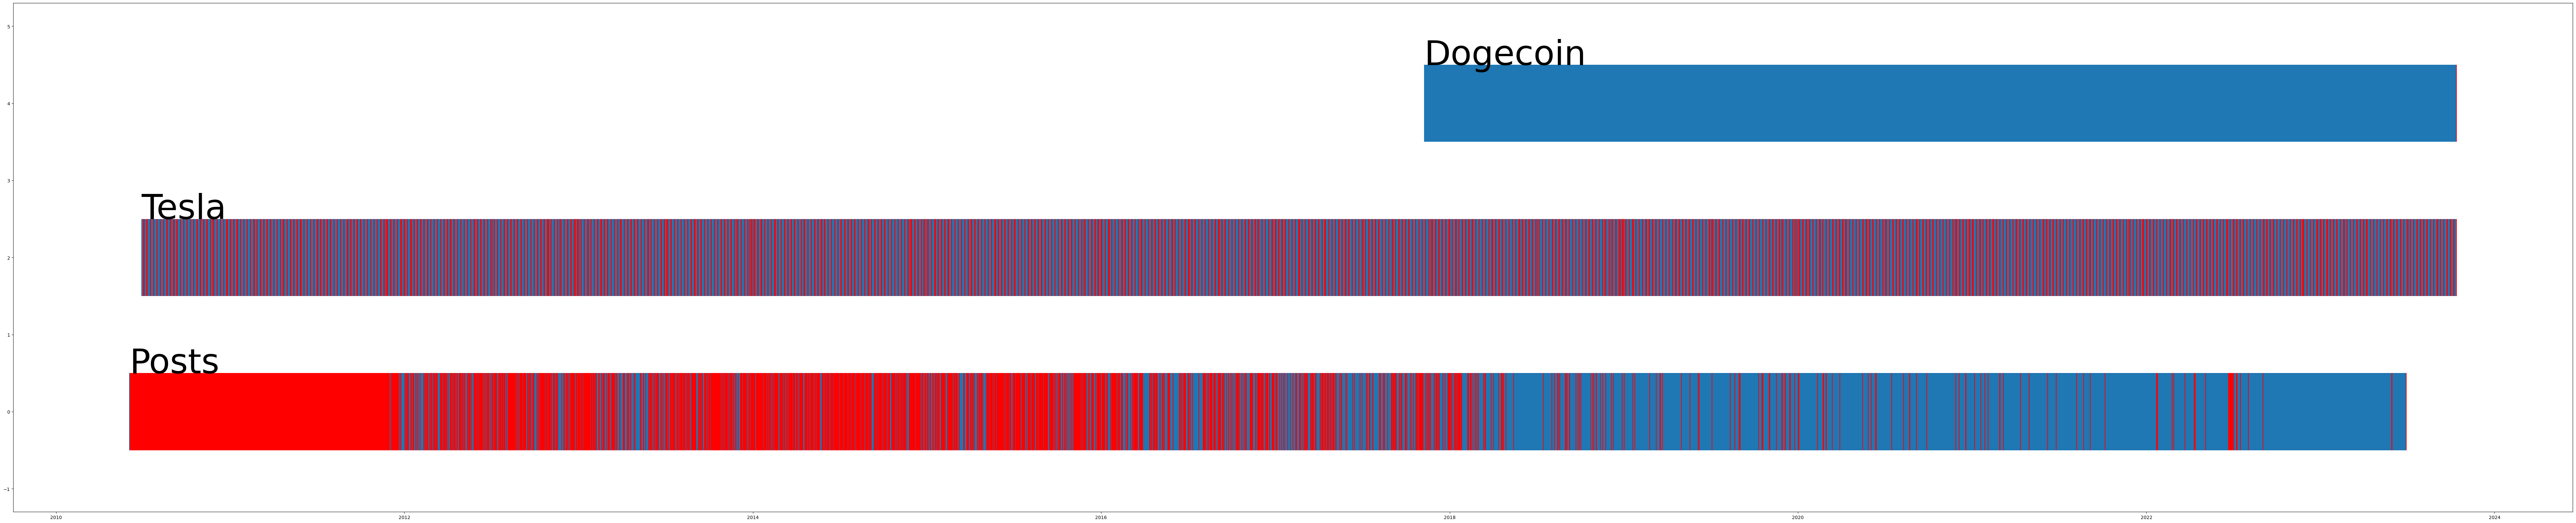
\includegraphics[width=.7\textwidth, height=100px]{../imgs/Dichte1.png}
	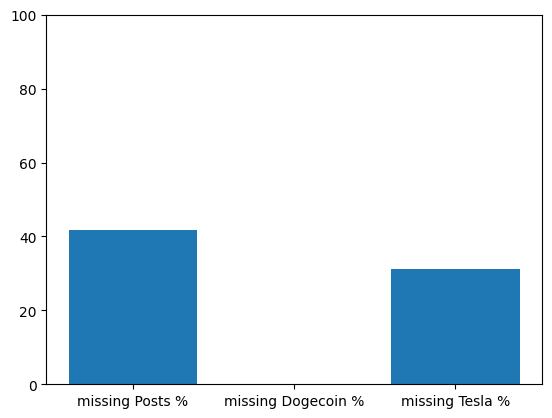
\includegraphics[width=.3\textwidth, height=100px]{../imgs/Dichte2.png}
 	\caption{Datendichte}
 	\label{fig:Datendichte}
\end{figure}
Die erste Grafik zeigt die gesamte Zeitspanne (04.06.2010 - 12.10.2023) aller gesammelter Daten aus den drei Datensätzen.
Dabei beschreibt der rote Anteil alle fehlenden Tage des jeweiligen Datensatzes.
Die Regelmäßigkeit der fehlenden Daten im Tesla-Datensatz kann auf die geschlossenen Tage der Aktienbörse zurückgeführt werden;
demzufolge, weist der Dogecoin-Datensatz auch keine fehlenden Datensätze auf, da die Kryptomärkte keiner Schließzeit unterliegen.
Die prozentuale Anzahl der fehlenden Tage kann der zweiten Grafik entnommen werden.
Darüber hinaus lässt sich aus dem Schaubild die Aussage ableiten, dass das Korrespondenzverhalten von Elon Musk auf der Plattform X über die Zeit zunimmt.
Zusammen mit der eineinhalbjährigen Pause nach seinem ersten Tweet am 04.06.2010 lässt dies die Vermutung offen, dass Musk erst nach und nach das Potenzial der Plattform erkannte, bis er diese schließlich am 04.04.2022 unter fragwürdigen Umständen aufkaufte. 
Die Auswertung der fehlenden Tage wird durch die Methode \textit{get\_density(df:pd.DataFrame)} ermöglicht, welche zunächst eine Liste aller Tage erstellt, die im jeweiligen Datensatz vorhanden sein sollten.
Im Folgenden wird ein neuer Datensatz erstellt, der alle Tage, sowie den entsprechenden booleschen Wert (1 vorhanden / 0 fehlend) für jeden Tag des zu untersuchenden Datensatzes enthält.
Dieser resultierende Datensatz kann nun mit einem Eventplot skizziert werden und bietet die Möglichkeit, den Prozentsatz der fehlenden Tage zu ermitteln.
\begin{python}
def get_density(df:pd.DataFrame):
    start_date = min(df["date"]).replace(hour=0, minute=0, second=0, microsecond=0)
    end_date = max(df["date"]).replace(hour=0, minute=0, second=0, microsecond=0) + pd.Timedelta(days=1)
    all_dates = pd.DataFrame({"date": pd.date_range(start_date, end_date, freq='D')})
    all_dates["exists"] = all_dates["date"].isin(df["date"]).astype(int)
    return all_dates
\end{python}


\subsection{Data Preperation} \label{Data Preperation}
Da die Datensätze schon sehr gut strukturiert sind, ist es nicht nötig eine erweiterte Data Preperation durchzuführen.
Optional könnten die ungenutzten Spalten entfernt werden, um Rechenzeit und Speichergröße zu verringern, jedoch ist beides unerheblich.



\section{Lösungsansatz} \label{Lösungsansatz} 


\subsection{Hilfsfunktionen} \label{Hilfsfunktionen}

\subsubsection{Intervallselektion} \label{Intervallselektion}
Die Methode \textit{check\_filter()} erkennt, ob in einem Text gewisse Schlüsselwörter aus einer Filter-Liste enthalten sind.
Dies ermöglicht das Filtern der Posts anhand der eventuell im Post-Text enthaltenen Schlüsselwörter (bspw.: \textit{Dogecoin}).
Dabei kann in Abhängigkeit der Variable \textit{hit}, entweder nach dem Vorhandensein (hit=True) oder dem Fehlen (hit=Flase) der Schlüsselwörter sortiert werden.
Dies geschieht, indem die Methode je nach Gegebenheit den booleschen Wert Wahr oder Falsch annimmt.
\par
Die Methode \textit{get\_Intervall} generiert das zu betrachtende Datensatz-Intervall, welches ausgehend von einem Startdatum die nächsten vorhandenen \textit{n} Tage aus einem Stock-Datensatz enthält.
Die Anzahl der Tage wird durch den Parameter \textit{intervall\_length} gegeben und beträgt standardmäßig den Wert 3.
Es wird außerdem berücksichtigt, dass das Startdatum nicht im Stock-Datensatz enthalten ist.
In diesem Fall nimmt das Unterprogramm das nächste vorhandene Datum.
Ausgehend von dem gefundenen Datum, werden der Start-Index sowie der End-Index des Datensatz-Ausschnittes berechnet.
Dabei wird ebenfalls berücksichtigt, dass das End-Datum ggf. auch nicht mehr im Datensatz erhalten ist. Trifft dies zu, so kann kein Intervall erstellt werden und es wird None zurückgegeben.
Dieser Fall ist jedoch bei unseren Datensätzen nicht zwingend zu berücksichtigen, da die Stock-Datensätze deutlich aktueller sind, als der Datensatz der Tweets, aus dem das Startdatum stammt.

\subsubsection{Kursverlauf} \label{Kursverlauf}
Die folgende Hilfsmethode \textit{get\_Trend} ist ein wichtiges Kernstück der Analyse und wird dazu verwendet, die Änderung des Aktienkurses im gegeben Intervall zu analysieren.
Dafür betrachten wir die Spalte \textit{close}, die dem täglichen Abschlusswert der Aktie entspricht.
Im Folgenden ermittelt die Methode mithilfe einer linearen Regression eine Gerade, welche das Wachstum der Aktie im gegebenen Zeitraum repräsentiert.
Anschließend werden mit diesem Modell die erwarteten Werte der Aktie für den ersten bzw. letzten Tag des zu betrachtenden Intervalls berechnet.
Zwischen diesen resultierenden Werten kann nun der prozentuale Unterschied kalkuliert werden.
Dies erfolgt nach der Rechenvorschrift, $ (day_{n} - day_{0}) / |day_{0}| * 100 $ wobei $day_{0}$ dem ersten Tag des Intervalls und $day_{n}$ dem letzten Tag des Intervalls entspricht. 
Dabei hat dieses Verfahren den Vorteil, dass alle Werte des Intervalls gleichermaßen berücksichtigt werden.

\newpage

\begin{python}
def get_trend(stock_part:pd.DataFrame):
    colses_of_Intervall:list = stock_part["close"].tolist()
    
    x = np.array(range(len(colses_of_Intervall))).reshape(-1, 1)
    y = np.array(colses_of_Intervall)

    model = LinearRegression().fit(x, y)

    x_first = np.array([0]).reshape(-1, 1)
    x_last = np.array([len(colses_of_Intervall) - 1]).reshape(-1, 1)

    y_first = model.predict(x_first)[0]
    y_last = model.predict(x_last)[0]

    change_percentage = round((y_last - y_first) / abs(y_first), 4) * 100

    return [change_percentage, model]
\end{python}
Die Hilfsmethode \textit{get\_Absolute} kann vernachlässigt werden, da sich unsere Analyse ausschließlich auf den Trend-Verlauf bezieht.
Dieser ist aufgrund der Berücksichtigung aller Werte des Intervalls weniger anfällig für extreme Außeneinfluss und unerwartete Schwankungen und eignet sich dadurch besser zur Beantwortung der Fragestellung.


\subsection{Hauptschleife} \label{Hauptschleife}
Die Hauptschleife umfasst die grundlegende Funktionalität zur Auswertung der Datensätze in Bezug auf die Fragestellung.
Aufgrund der hohen Komplexität des Vorgangs konnte nicht auf eine Funktionskombination bestehender APIs zurückgegriffen werden.
Somit musste die Funktion von Grund auf neu entwickelt werden.
Dafür wird ein neuer Datensatz \textit{influence} erstellt, welcher alle Tage, an denen ein Post mit den entsprechenden Filterkriterien verfasst wurde, umfasst.
Für jeden dieser Tage wird das Datum, eine Liste aller Posts, die Anzahl dieser Posts, sowie der in \ref{Kursverlauf} errechnete Kursverlauf aufgezeichnet.
So iteriert diese Schleife zunächst über alle Tweets, die im Datensatz \textit{Posts} enthalten sind.
Im Anschluss wird nun durch die Methode \textit{check\_filter} überprüft, ob die aktuelle Zeile den Filtern gerecht wird.
Trifft dies nicht zu, so wird diese Zeile direkt übersprungen.
Ansonsten wird das Datum aus der aktuellen Zeile ausgelesen.
Im Folgenden wird überprüft, ob der aktuelle Tag schon im Datensatz \textit{influence} enthalten ist, was zutrifft, wenn an einem Tag mehrere Posts vorliegen.
Ist dies der Fall, so wird dieser nur um den aktuellen Posttext ergänzt, sowie die Anzahl der Posts an diesem Tag inkrementiert.
Ist dieser Tag noch nicht im Datensatz \textit{influence} enthalten, so wird für den aktuellen Tag zunächst das Intervall des Stock-Datensatzes bestimmt.
Ist dies nicht möglich, weil ggf. Daten fehlen, wird eine Warnung ausgegeben und die Schleife fährt fort.
Dies ist jedoch wie in \ref{Intervallselektion} beschrieben zu vernachlässigen.
Wenn das Intervall erfolgreich erstellt wurde, werden nun alle Berechnungen der beiden Hilfsfunktionen auf dieses angewandt.
Schlussendlich werden alle Werte unter diesem Tag in den Datensatz \textit{influence} eingefügt.
Hat die Schleife alle Posts abgearbeitet, kann dieser Datensatz zurückgegeben werden.
Zudem wird der prozentuale Anteil der im \textit{influence} enthaltenen Posts von allen Posts ermittelt und mit zurückgegeben.
\newpage
\begin{python}
def get_influence(stock:pd.DataFrame, posts:pd.DataFrame=Posts, filter_list:list=[], hit:bool=False,):
    # find a common start date
    start_date = max(posts['date'].min(), stock['date'].min())
    # adjust Posts to startdate
    posts = posts[posts['date'] >= start_date]
    # adjust Stock to startdate
    stock = stock[stock['date'] >= start_date]

    influence:pd.DataFrame = pd.DataFrame(columns=['date', 'posts', 'count_posts', 'trend', 'absolute'])
    j = 0
    old_date = None
    for i, post in posts.iterrows():
        if not check_filter(str(post['text']), filter_list, hit=hit):
            continue
        else:
            date = pd.to_datetime(post['date']).normalize()
            if not date == old_date:
                Intervall = get_Intervall(date, stock)
                if Intervall is None:
                    print("No Data Available")
                    continue
                cp_trend, model = get_trend(Intervall)
                cp_absolute = get_absolute(Intervall)
                influence.loc[j] = [date] + [[post['text']]] + [0] + [cp_trend] + [cp_absolute]
                old_date = date
                j += 1
            else:
                influence.loc[j-1, 'posts'].append(post['text'])
                influence.loc[j-1, 'count_posts'] += 1
    return [influence, j/i*100]
\end{python}



\subsection{Erzeugung} \label{Erzeugung}
Im Folgenden können nun beliebig viele Influence-Datensätze für eine Analyse erstellt werden.
Dafür wird eine Filter-Liste mit den entsprechenden Schlüsselwörtern der Funktion \textit{get\_influence} übergeben.
Außerdem kann optional das zu betrachtende Zeitintervall beliebig angepasst werden.


\newpage

\section{Auswertung} \label{Auswertung}

\subsection{Posts} \label{Posts}

\subsubsection{Verteilung} \label{Verteilung}
\begin{figure}[h]
  	\centering
  	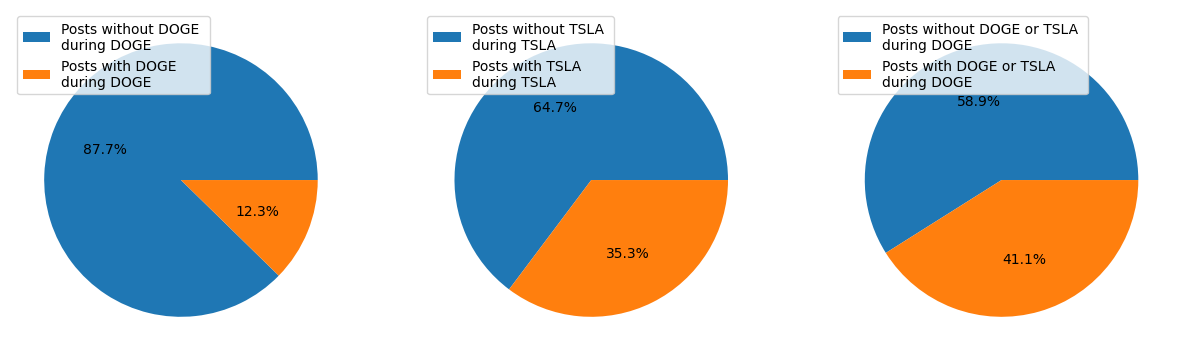
\includegraphics[width=\textwidth]{../imgs/Verteilung.png}
 	\caption{Verteilung}
 	\label{fig:Verteilung}
\end{figure}
Dieses Diagramm zeigt die Verteilung der entsprechenden Schlüsselwörter in allen Posts des zu betrachtenden Zeitraums.
Dabei ist es wichtig zu beachten, dass der zu betrachtende Zeitraum zusammen mit den Aufzeichnungen des Kursverlaufs beginnt.
Demzufolge wird beispielsweise die Verteilung der Schlüsselwörter für Dogecoin nur für den Zeitraum des Dogecoin-Datensatzes erstellt.
Interessant ist hierbei die Tatsache, dass Elon Musk fast doppelt so viel über Tesla twittert als über Dogecoin.
Insbesondere wenn man sich die kombinierten Schlüsselwörter über den Zeitraum des Dogecoin-Datensatzes (da Dogecoin-Datensatz \textless Tesla-Datensatz, siehe Abbildung \ref{fig:Verteilung}) näher anschaut, ist deutlich zu erkennen, dass selbst hier Tesla einen Anteil von 28,8 \% besitzt (da 41,1 \%-12,3 \%).
Dies ist immer noch mehr als doppelt so viel als die 12,3 \% der Dogecoin-Posts.
Dies könnte daran liegen, dass Dogecoin von Elon Musk mehr als eine Art Neben- oder Spaßprojekt angesehen wird; seine Verbundenheit zu Tesla ist auch schon alleine durch seine Position als CEO gegeben.

\subsubsection{Verlauf} \label{Verlauf}
\begin{figure}[!htb]
  	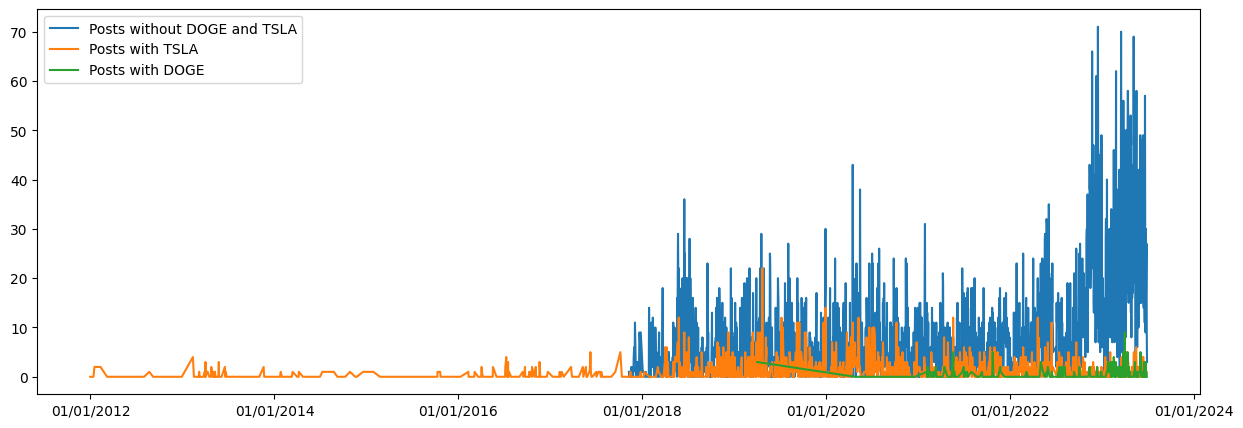
\includegraphics[width=\textwidth, center]{../imgs/Verlauf.png}
 	\caption{Verlauf}
 	\label{fig:FigVerlauf}
\end{figure}
Dieses Diagramm zeigt den Tag (x-Achse), sowie die Anzahl der Posts an diesem Tag (y-Achse). Auch hier sieht man die in \ref{Data Understanding} aufgeworfene These, dass das Korrespondenzverhalten von Elon Musk im Verlauf der Zeit zunimmt.
Zudem wird diese Vermutung nun auch durch die Anzahl der Posts an einem Tag gestützt.
Denn dieser ist zu entnehmen, dass Elon Musk nicht nur an mehreren Tagen, sondern vor allem auch deutlich häufiger pro Tag tweetet.
Dieses Verhalten kann insbesondere seit der Übernahme der Plattform am 04.04.2022 beobachtet werden.
Während im Sommer 2019 ein Großteil seiner Posts die Schlüsselwörter von Tesla beinhalteten, postet Elon Musk mittlerweile schon fast genau so viel über Dogecoin wie über Tesla. Das könnte ein Indiz dafür sein, dass Dogecoin für Musk zurzeit an Interesse gewonnen hat.

\subsubsection{Zusammenhänge} \label{Zusammenhänge}
\begin{figure}[!htb]
	

    		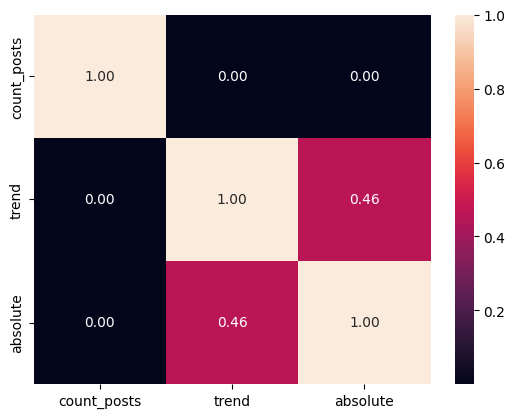
\includegraphics[width=0.5\textwidth, center]{../imgs/Korrelation.png}
    		\caption{Korrelation}
    		\label{fig:Korrelation}

	
		
\end{figure}

Der wichtigste Aspekt, der der Korrelationstabelle des Einfluss-Datensatzes entnommen werden kann, ist die Unabhängigkeit zwischen der Spalte \textit{count\_posts} und den Werten \textit{trend} und \textit{absolute}.
	Dies zeigt, dass die Anzahl der Posts (Tweets) an einem Tag keinen Einfluss auf den Verlauf der beiden Wertpapiere hat.
	Die Korrelationstabelle wurde unter Verwendung der Bibliothek Seaborn aus der Vereinigung der Schlüsselwort freien Einfluss-Datensatz erstellt.
	\begin{python}
	influences_corr = pd.concat(
	    [
	        influences_t_d[['count_posts', 'trend', 'absolute']],
	        influences_t_t[['count_posts', 'trend', 'absolute']]
	    ]
	).corr()
	sns.heatmap(influences_corr, annot=True, fmt=".2f")
	plt.show()
	\end{python}

\newpage

\subsection{Verlauf} \label{VerlaufSub}

\subsubsection{i=3} \label{i=3}
\begin{figure}[!htb]
  	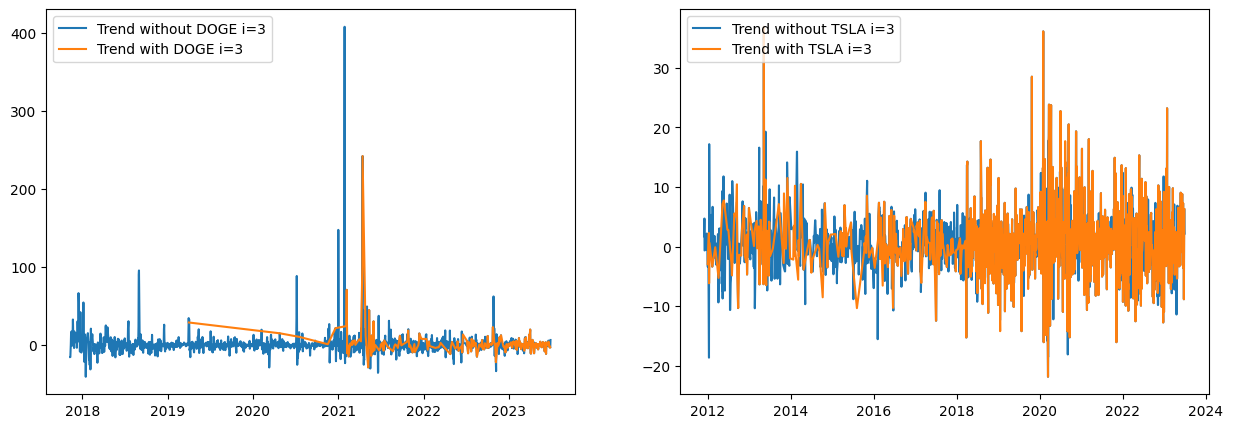
\includegraphics[width=\textwidth, center]{../imgs/Trendi3.png}
 	\caption{Trend i=3}
 	\label{fig:Trendi3}
\end{figure}
Die analysierten Diagramme zeigen den Einfluss der nächsten 3 Tage von Elon Musks Posts auf die Kursentwicklung von Dogecoin und Tesla. Bezüglich Dogecoin fällt auf, dass Musks Tweets meist nur geringfügige Auswirkungen zu haben scheinen, da die prozentualen Veränderungen im Vergleich zu den Trends ohne das Stichwort Doge oft relativ gering sind. Es gibt sogar Situationen, in denen die Trends ohne Musks Tweets deutlich stärkere Veränderungen aufweisen als mit. Jedoch ist auch erkennbar, dass Musk erst ab Mitte 2022 aktiv über Dogecoin twittert.
Im Fall von Tesla hingegen ist erkennbar, dass Musks Tweets einen deutlich stärkeren Einfluss auf den Aktienverlauf haben. Insbesondere ab 2018 ist eine Zunahme seiner Tweets zu beobachten. Die Diagramme zeigen Spitzen, bei denen ein Tweet den Trend sowohl positiv als auch negativ beeinflusst. Dennoch verläuft der Trend größtenteils ähnlich, ob mit oder ohne einen entsprechenden Tweet. Dies legt nahe, dass Musk zwar in der Lage ist, den Aktienkurs von Tesla durch seine Tweets zu beeinflussen, aber dass auch andere, uns unbekannte Faktoren eine bedeutende Rolle spielen.
In den meisten Fällen scheint sich die Aktie so zu verhalten, als ob Musks Tweets den Markt nicht wesentlich beeinflussen würden. Dennoch gibt es bestimmte Punkte, an denen Musk in der Lage ist, den Trend der Aktie stark zu beeinflussen. Dabei bleibt jedoch unklar, ob diese Veränderungen gezielt geplant sind oder eher Zufälle sind.

\subsubsection{i=5} \label{i=5}
\begin{figure}[!htb]
  	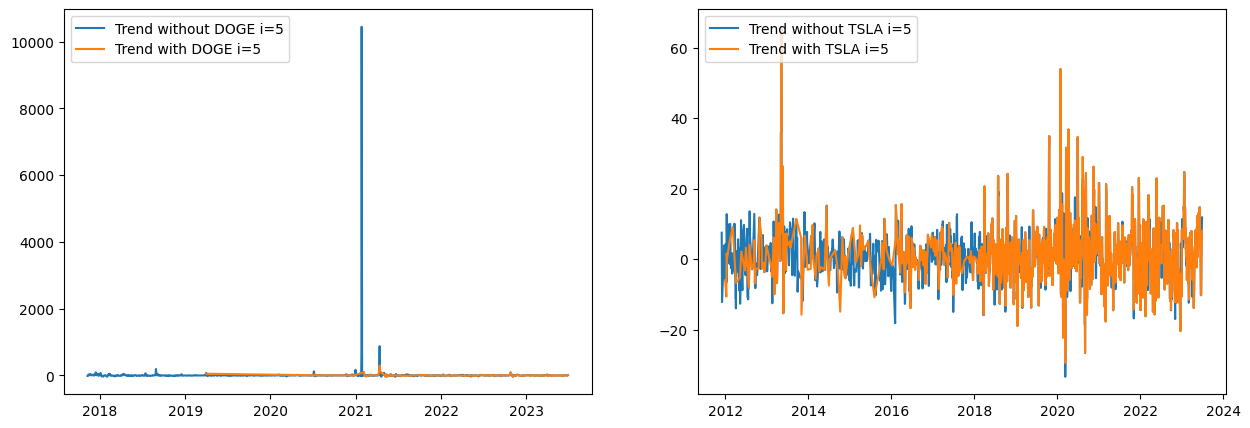
\includegraphics[width=\textwidth, center]{../imgs/Trendi5.png}
 	\caption{Trend i=5}
 	\label{fig:Trendi5}
\end{figure}
Der Unterschied dieser Diagramme zu den vorherigen ist einzig die Änderung der betrachteten Zeitspanne. Jedoch ist erkennbar, dass, vor allem bei Dogecoin, sich der Einfluss auf den Trend stark verändert. Der Höhepunkt Anfang 2021, der die Veränderung des Trends von Dogecoin ohne einen Tweet über Dogecoin zeigt, ist in dieser Ansicht noch höher. Aufgrund dieses Höhepunktes ist es kaum möglich, mit bloßem Auge den restlichen Graphen auszuwerten. Auch bei Tesla sind kleinere Abweichungen zu erkennen. Vor allem haben die Tweets von Musk über Tesla einen höheren Einfluss, aber der Trend ohne einen Tweet verstärkt sich. Es scheint trotzdem so, als ob der Trend in den ersten 3 Tagen stärker beeinflusst wird. Das lässt darauf schließen, dass sich der Trend nach 3 Tagen wieder langsam verflüchtigt.


\subsubsection{Durchschnitt} \label{Durchschnitt}
\begin{figure}[!htb]
  	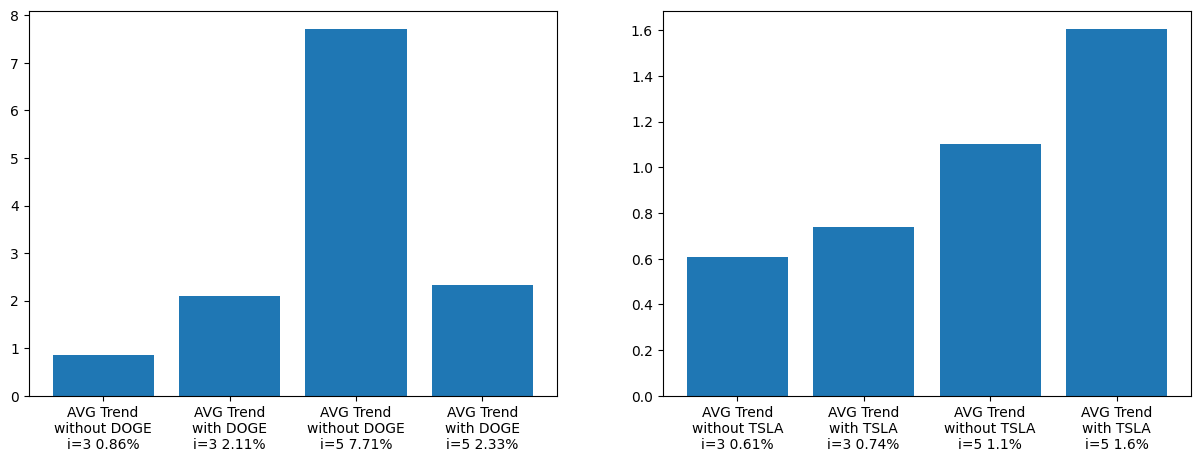
\includegraphics[width=\textwidth, center]{../imgs/Trend_Durchschnitt.png}
 	\caption{Trend Durchschnitt}
 	\label{fig:Trend Durchschnitt}
\end{figure}
In diesen Grafiken werden Tesla und Dogecoin anhand des Durchschnitts in verschiedenen Zeitintervallen verglichen. In beiden Fällen wird einmal der Trend genommen, ohne, dass Elon Musk das Wort \textit{Tesla} oder \textit{Dogecoin} in seinen Tweets genutzt hat und einmal, wenn er es verwendet hat.
In der linken Grafik wird auf die Dogecoin Aktie geschaut, bei Tweets ohne die Verwendung des Wortes \textit{Dogecoin} und mit der Verwendung des Wortes \textit{Dogecoin}. Im Fall von i = 3 ist der Durchschnitt ohne die Verwendung des Wortes \textit{Dogecoin} bei 0,86 \% und mit dem Wort \textit{Dogecoin} bei 2,11 \%. Im Fall von i = 5 ist der Durchschnitt ohne die Verwendung des Wortes \textit{Dogecoin} bei 7,71 \% und mit dem Wort \textit{Dogecoin} bei 2,33 \%. Hieraus kann man schließen, dass die Tweets auf einen kürzeren Zeitraum einen stärkeren Einfluss haben und nach mehreren Tagen wieder abflacht.
In der rechten Grafik wird auf die Tesla Aktie geschaut, bei Tweets ohne die Verwendung des Wortes \textit{Tesla} und mit der Verwendung des Wortes \textit{Tesla}. Im Fall von i = 3 ist der Durchschnitt ohne die Verwendung des Wortes \textit{Tesla} bei 0,61 \% und mit dem Wort \textit{Tesla} bei 0,74 \%. Im Fall von i = 5 ist der Durchschnitt ohne die Verwendung des Wortes \textit{Tesla} bei 1,1 \% und mit dem Wort \textit{Tesla} bei 1,6 \%. Hieraus kann man schließen, dass die Tweets auf einen Zeitraum von i = 5 Tagen einen stärken Einfluss haben. 

\section{Gesamtbewertung / Erwartung} \label{Gesamtbewertung / Erwartung}

\subsection{Die Legalität} \label{Die Legalität}
Die Legalität und die Auswirkung von Elon Musks Tweets auf den Aktienmarkt sind ein komplexes Thema. Normalerweise müssen Äußerungen insbesondere von einflussreichen Personen, Managern und Geschäftsführern von börsenorientierten Unternehmen in dem Rahmen der geltenden Gesetze und Vorschriften erfolgen.
Die SEC (Securities and Exchange Commission) hat spezifische Regeln für Offenlegungen durch Direktoren börsennotierter Unternehmen. Der Zweck dieser Regeln besteht darin, sicherzustellen,
dass relevante Informationen fair und gleichzeitig für alle Marktteilnehmer zugänglich sind. Musk und Tesla standen in der Vergangenheit unter Beobachtung der SEC, insbesondere aufgrund von Elon Musks Tweets über Tesla. Einige von Musks Tweets wurden als potenzielle Verstöße gegen die SEC-Regeln angesehen, dazu gehörte unter anderem ein Tweet aus dem August 2018, in dem er darüber spekulierte, ob er Tesla von der Börse nehme, was zu Rechtsstreitigkeiten und Vergleichen in einer Höhe von bis zu 20 Millionen Dollar mit der SEC führte. Es ist wichtig zu beachten, dass die Rechtslage in solchen Fällen weitgehend von den konkreten Umständen und den geltenden Gesetzen abhängt. Musk und sein Unternehmen müssen sich noch mit der öffentlichen Kommunikation und ihren Auswirkungen auf den Aktienmarkt befassen.

\subsection{Investitionsempfehlungen} \label{Investitionsempfehlungen}
Anhand unserer Auswertungen und Grafiken kann man sehen, dass Dogecoin tendenziell eher Kurzzeitmuster aufzuweisen hat, nachdem Elon Musk in seinen Tweets die Kryptowährung erwähnt hat. Bei Dogecoin sieht man, dass der Preis zeitweise deutlich steigt, gefolgt von Phasen, in denen sich der Trend wieder abflacht oder abwärts bewegt. Generell kann man sagen, dass hier eher Investments in einem Zeitraum von circa 3 Tagen sinnvoll sind. Bei der Tesla Aktie kann man anhand unserer Auswertung eher einen Zeitraum von 5 Tagen empfehlen.


\section{Fazit} \label{Fazit}
Anhand der Erkenntnisse, die wir aus den jeweiligen Auswertungen erlangt haben, können wir die genaue Fragestellung beantworten. Bezüglich der Legalität der Einflussnahme von Elon Musk auf den Aktienmarkt kann man sagen, dass er sich an der Grenze des rechtlichen Rahmens bewegt und auch schon in manchen Fällen über diese Grenze hinweg gegangen ist. Grundsätzlich ist es nur im Rahmen der Gesetze möglich, für Personen, die sehr viel Einfluss haben, Äußerungen zu tätigen. Besonders auf Social-Media-Plattformen wie X (ehemals Twitter) ist eine Einflussnahme auf den Aktienmarkt gesetzlich nicht erlaubt. Elon Musk ist eine dieser einflussreichen Personen und daher hat auch er die Pflicht, sich an diese Vorschriften zu halten.
Welchen Einfluss seine Äußerungen auf Social Media schlussendlich wirklich haben, konnten wir ebenfalls herausfinden. Anhand unserer Beobachtungen, dass der Trend und die absoluten Werte der Aktie Tesla sich immer wieder durch Musk beeinflussen lassen, schließen wir, dass Musk durchaus den Kursverlauf von Tesla relativ stark beeinflusst. Jedoch nur meist gemäßigt und nur selten stark. Dieses Verhalten lässt sich mit der Legalität begründen, denn so überschreitet Musk nicht die Grenze.
Auf Dogecoin hat Musk zwar weniger Einfluss, aber auch hier übt er diesen immer wieder aus. Um als Privatperson auf solch einen Einfluss besser vorbereitet zu sein, könnte man nun das Programm noch so erweitern, dass es eine Zukunftsvorhersage berechnet und ausgibt. Aufgrund dieser Vorhersagen kann man dann seine Investments besser planen und durchführen. Aus zeitlichen Gründen war uns nur die Auswertung möglich, wie der Trend sich allgemein verändert, wenn Musk etwas mit Tesla oder Dogecoin postet. Aufgrund dieser Auswertung kann man nicht automatisch nach einem neuen Post sagen, wie der Kurs sich nun verhalten wird. Eine Programmerweiterung könnte, wenn man genauer anschaut, was gepostet wird, dieses Problem beheben und fundierte Vorhersagen erstellen.
\end{document}
